\documentclass{dlproblemset}
\usepackage{tikz}
\usetikzlibrary{positioning}
\tikzset{every picture/.style={line width=0.75pt}}

% ---- Estilos das unidades no diagrama da rede de Perceptrons com fronteira em V ----
\tikzset{
  mlpunit/.style={circle, draw, minimum size=7mm, inner sep=0pt, font=\scriptsize},
  mlpin/.style={font=\scriptsize},
  mlpw/.style={font=\tiny, inner sep=1.2pt}
}

% ---- Região classificada como +1 nas alternativas da questão da rede de Perceptrons com fronteira em V ----
% Quadrado [0,4] x [0,4]; #1 é o polígono sombreado.
\newcommand{\regpanel}[1]{%
\begin{tikzpicture}[scale=0.64, baseline=(current bounding box.center)]
  \begin{scope}
    \clip (0,0) rectangle (4,4);
    \fill[black!18] #1;
  \end{scope}
  \foreach \g in {1,2,3} { \draw[gray!35] (\g,0) -- (\g,4); \draw[gray!35] (0,\g) -- (4,\g); }
  \draw[gray!70] (0,0) rectangle (4,4);
  \foreach \t in {0,1,2,3,4} { \node[font=\tiny, below, inner sep=1.5pt] at (\t,0) {$\t$}; \node[font=\tiny, left, inner sep=1.5pt] at (0,\t) {$\t$}; }
  \node[font=\scriptsize, below] at (2,-0.55) {$x_1$};
  \node[font=\scriptsize, left] at (-0.55,2) {$x_2$};
\end{tikzpicture}}

\title{Perceptron}
\subtitle{Lista de Exercícios}

\begin{document}

\begin{enumerate}[1)]

    \item Por que o \textit{Perceptron} como proposto originalmente ($\hat{y}^{(i)} = sign(\mathbf{X}^{(i)}\boldsymbol{\theta})$) não pode ser organizado em uma rede para formar um \textit{Multi Layer Perceptron}?
    \begin{enumerate}[(a)]
        \item Pois a derivada da função de ativação em relação aos pesos ou é igual a zero ou indefinida.
        \item Pois o \textit{dot product} dos pesos com as \textit{features} não pode ser derivado.
        \item Pois \textbf{apenas} a descontinuidade na função de ativação $sign(x)$ em $x = 0$ impede o processo de otimização via descida de gradiente.
        \item Pois o perceptron possui a limitação de modelar apenas problemas que são linearmente separáveis.
    \end{enumerate}
    %a

    \item Por que uma rede de Perceptrons de Rosenblatt não pode ser treinada via descida de gradiente e \textit{backpropagation}?

    \item Prove que um Perceptron com duas entradas $\hat{y}=sinal(\theta_0 + X_1\theta_1 + X_2\theta_2)$ gera uma fronteira de decisão linear.

    \item Crie um Perceptron que se comporta como uma função \textit{and}.

    \item Por que uma rede de Perceptrons de Rosenblatt, na sua formulação original com saída $\hat{y} = \mathrm{sign}(\mathbf{x}^\top \boldsymbol{\theta})$, não pode ser organizada em uma rede multicamadas treinada por descida de gradiente e \textit{backpropagation}?
    \begin{enumerate}[(a)]
        \item Porque o produto escalar $\mathbf{x}^\top \boldsymbol{\theta}$ não é diferenciável em relação aos pesos $\boldsymbol{\theta}$.
        \item Porque a derivada de $\mathrm{sign}(z)$ é zero em $z \neq 0$ e indefinida em $z = 0$, bloqueando a regra da cadeia.
        \item Porque o Perceptron tem como limitação modelar apenas problemas linearmente separáveis; com função de ativação contínua, esse problema desapareceria automaticamente.
        \item Porque a função $\mathrm{sign}$ é descontínua, o que impede que a função de custo de entropia cruzada seja calculada.
        \item Porque a regra de atualização original do PLA (\textit{Perceptron Learning Algorithm}) é incompatível com descida de gradiente; basta substituir o PLA pelo SGD para o problema desaparecer.
        \item Porque o número de parâmetros do Perceptron é grande demais para ser otimizado por descida de gradiente em hardware atual.
        \item Porque o Perceptron já realiza descida de gradiente internamente; encadeá-los em rede multicamadas dobraria a operação e levaria a divergência.
        \item Porque a saída $\hat{y} \in \{-1, +1\}$ não é interpretável como probabilidade, e a descida de gradiente exige saídas probabilísticas.
    \end{enumerate}
    %b

    \item Considere um Perceptron de Rosenblatt com duas entradas $X_1, X_2 \in \{-1, +1\}$ e saída $\hat{y} = \mathrm{sinal}(\theta_0 + \theta_1 X_1 + \theta_2 X_2)$, em que $\mathrm{sinal}(z) = +1$ se $z \geq 0$ e $-1$ caso contrário. Codificando \emph{verdadeiro} como $+1$ e \emph{falso} como $-1$, qual configuração de pesos $(\theta_0, \theta_1, \theta_2)$ implementa a porta lógica \textbf{OR}, isto é, $\hat{y} = +1$ se e somente se $X_1 = +1$ ou $X_2 = +1$?
    \begin{enumerate}[(a)]
        \item $(\theta_0, \theta_1, \theta_2) = (-3,\ 1,\ 1)$
        \item $(\theta_0, \theta_1, \theta_2) = (-1,\ -1,\ -1)$
        \item $(\theta_0, \theta_1, \theta_2) = (-1,\ 1,\ 1)$
        \item $(\theta_0, \theta_1, \theta_2) = (1,\ 1,\ 1)$
        \item $(\theta_0, \theta_1, \theta_2) = (1,\ 1,\ -1)$
        \item $(\theta_0, \theta_1, \theta_2) = (1,\ -1,\ -1)$
        \item $(\theta_0, \theta_1, \theta_2) = (-1,\ 1,\ -1)$
        \item $(\theta_0, \theta_1, \theta_2) = (3,\ 1,\ 1)$
    \end{enumerate}
    %d

    \item Na rede abaixo, cada círculo é uma unidade que aplica $\mathrm{sinal}$ à soma ponderada das suas entradas somada ao viés indicado \emph{dentro} do círculo, e os números sobre as arestas são os pesos. Considere $\mathrm{sinal}(z) = +1$ para $z \geq 0$ e $\mathrm{sinal}(z) = -1$ para $z < 0$.

    \begin{center}
    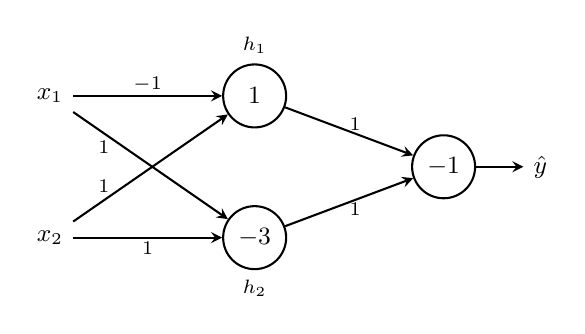
\begin{tikzpicture}[>=stealth,
        mlpunit/.style={circle, draw, minimum size=8mm, inner sep=0pt, font=\small},
        mlpin/.style={font=\small}, mlpw/.style={font=\scriptsize, inner sep=1.2pt}]
      \node[mlpin]   (x1) at (0,0.9)   {$x_1$};
      \node[mlpin]   (x2) at (0,-0.9)  {$x_2$};
      \node[mlpunit] (h1) at (2.6,0.9)  {$1$};
      \node[mlpunit] (h2) at (2.6,-0.9) {$-3$};
      \node[mlpunit] (o)  at (5.0,0)    {$-1$};
      \node[font=\scriptsize, above=0pt of h1] {$h_1$};
      \node[font=\scriptsize, below=0pt of h2] {$h_2$};
      \node[mlpin, right=0.6cm of o] (yh) {$\hat{y}$};
      \draw[->] (x1) -- node[mlpw, above]{$-1$} (h1);
      \draw[->] (x2) -- node[mlpw, pos=0.25, above left=-1pt]{$1$} (h1);
      \draw[->] (x1) -- node[mlpw, pos=0.25, below left=-1pt]{$1$} (h2);
      \draw[->] (x2) -- node[mlpw, below]{$1$} (h2);
      \draw[->] (h1) -- node[mlpw, above right=-2pt]{$1$} (o);
      \draw[->] (h2) -- node[mlpw, below right=-2pt]{$1$} (o);
      \draw[->] (o) -- (yh);
    \end{tikzpicture}
    \end{center}

    Em qual dos gráficos abaixo a região sombreada corresponde exatamente ao conjunto de pontos $(x_1, x_2)$ classificados como $\hat{y} = +1$?

    \begin{center}
    \setlength{\tabcolsep}{1pt}
    \scalebox{0.93}{%
    \begin{tabular}{r@{\,}lr@{\,}lr@{\,}lr@{\,}l}
    \textbf{(a)} & \regpanel{(0,0) -- (1,0) -- (2,1) -- (3,0) -- (4,0) -- (4,4) -- (0,4) -- cycle} &
    \textbf{(b)} & \regpanel{(0,0) -- (4,0) -- (4,3) -- (2,1) -- (0,3) -- cycle} &
    \textbf{(c)} & \regpanel{(0,3) -- (1,2) -- (3,4) -- (0,4) -- cycle} &
    \textbf{(d)} & \regpanel{(2,1) -- (4,3) -- (4,0) -- (3,0) -- cycle} \\[0.5em]
    \textbf{(e)} & \regpanel{(2,1) -- (0,3) -- (0,0) -- (1,0) -- cycle} &
    \textbf{(f)} & \regpanel{(0,0) -- (1,0) -- (4,3) -- (4,4) -- (0,4) -- cycle} &
    \textbf{(g)} & \regpanel{(0,3) -- (2,1) -- (4,3) -- (4,4) -- (0,4) -- cycle} &
    \textbf{(h)} & \regpanel{(1,0) -- (2,1) -- (3,0) -- cycle} \\
    \end{tabular}
    }
    \end{center}
    %g

\end{enumerate}

\newpage

\subsection*{Gabarito}
\color{blue}
\begin{enumerate}[1)]

    \item a. A derivada da função $sign$ é zero em todo ponto onde é definida (e indefinida em $x=0$), então nenhum gradiente flui pelas unidades e o \textit{backpropagation} não tem como atualizar os pesos. A alternativa (c) erra ao afirmar que \textbf{apenas} a descontinuidade em $x=0$ impede a otimização, pois a derivada nula no restante do domínio também impede; (d) é uma limitação verdadeira do Perceptron isolado, mas não é o que impede organizá-lo em rede.

    \item Pois a derivada da função de ativação sinal é zero ou indefinida em todo domínio da função. Devido a isso, não conseguimos propagar os erros.

    \item A fronteira de decisão é o conjunto de pontos onde o argumento da função sinal troca de sinal, isto é, onde $\theta_0 + X_1\theta_1 + X_2\theta_2=0$. Supondo $\theta_2 \neq 0$, isolamos $X_2 = -\frac{\theta_0 + \theta_1 X_1}{\theta_2}$, que é a equação de uma reta no plano $(X_1, X_2)$ com coeficiente angular $-\theta_1/\theta_2$ e intercepto $-\theta_0/\theta_2$. De um lado dessa reta a saída é $+1$ e do outro é $-1$, portanto a fronteira de decisão é linear.

    \item $\hat{y}=sinal(\theta_0 + X_1\theta_1 + X_2\theta_2)$, onde $\theta_0=-1$, $\theta_1=1$, $\theta_2=1$ e as entradas falsas são codificadas como $-1$ e as entradas verdadeiras como $+1$. Verificação nas quatro combinações: $(-1,-1)\!: z=-3 \Rightarrow -1$; $(+1,-1)\!: z=-1 \Rightarrow -1$; $(-1,+1)\!: z=-1 \Rightarrow -1$; $(+1,+1)\!: z=+1 \Rightarrow +1$, exatamente a tabela-verdade do \textit{and}.

    \item b. A função $\mathrm{sign}(z)$ é constante em $\mathbb{R}^- \setminus \{0\}$ e em $\mathbb{R}^+ \setminus \{0\}$ (logo, derivada $0$) e descontínua em $z = 0$ (derivada indefinida). O \textit{backpropagation} multiplica gradientes camada a camada via regra da cadeia; com derivada zero em quase todo ponto, esses gradientes morrem e os pesos não são atualizados. A correção que historicamente viabilizou MLPs treináveis foi substituir $\mathrm{sign}$ por funções com derivada não nula (sigmoide, tanh, ReLU). Em (a), o produto escalar é trivialmente diferenciável em $\boldsymbol{\theta}$, a obstrução está na ativação; em (c), a separabilidade linear é uma limitação de capacidade do Perceptron único, que não desaparece automaticamente e não é o motivo de o gradiente não funcionar; em (d), a obstrução é da derivada (regra da cadeia), não da função de custo; em (e), a regra do PLA não tem ligação direta com a derivada da ativação, e trocar PLA por SGD ainda esbarra na derivada zero do $\mathrm{sign}$; em (f), o número de parâmetros é irrelevante para a derivabilidade; em (g), o PLA é uma regra de atualização específica do Perceptron, distinta da descida de gradiente; em (h), a interpretação probabilística é uma propriedade desejável da saída, não uma exigência da descida de gradiente.

    \item d. Com a codificação $\pm 1$ e viés $\theta_0$, basta avaliar $z = \theta_0 + \theta_1 X_1 + \theta_2 X_2$ nas quatro combinações de entrada. Para $(\theta_0, \theta_1, \theta_2) = (1, 1, 1)$: $(-1,-1)\!: z = -1 \Rightarrow \hat{y} = -1$; $(+1,-1)\!: z = 1 \Rightarrow +1$; $(-1,+1)\!: z = 1 \Rightarrow +1$; $(+1,+1)\!: z = 3 \Rightarrow +1$, exatamente a tabela-verdade do OR: falso apenas quando as duas entradas são falsas. Geometricamente, a fronteira $X_1 + X_2 = -1$ separa o ponto $(-1,-1)$ dos outros três. Em (a), $(-3, 1, 1)$ dá $z < 0$ em todas as combinações e a saída é constante em $-1$ (sempre falso); (b) $(-1, -1, -1)$ implementa o NOR, respondendo $+1$ apenas em $(-1,-1)$; (c) $(-1, 1, 1)$ implementa o AND, exigindo as duas entradas em $+1$, o erro clássico de deslocar a fronteira para o lado errado; (e) $(1, 1, -1)$ implementa $X_1 \lor \lnot X_2$ e falha em $(-1, +1)$; (f) $(1, -1, -1)$ implementa o NAND, respondendo $-1$ em $(+1,+1)$; (g) $(-1, 1, -1)$ implementa $X_1 \land \lnot X_2$, respondendo $+1$ apenas em $(+1,-1)$; (h) $(3, 1, 1)$ dá $z > 0$ em todas as combinações e a saída é constante em $+1$ (sempre verdadeiro).

    \item g. As unidades ocultas calculam $h_1 = \mathrm{sinal}(1 - x_1 + x_2)$, que vale $+1$ acima (e sobre) da reta $x_2 = x_1 - 1$, e $h_2 = \mathrm{sinal}(-3 + x_1 + x_2)$, que vale $+1$ acima da reta $x_2 = 3 - x_1$. As retas se cruzam em $(2;\ 1)$. A saída calcula $\mathrm{sinal}(-1 + h_1 + h_2)$; como $h_1 + h_2 \in \{2, 0, -2\}$, ela só vale $+1$ quando $h_1 = h_2 = +1$, isto é, a saída é um E lógico. A região positiva é a interseção dos dois semiplanos superiores, um V com vértice em $(2;\ 1)$ aberto para cima, que é o gráfico (g). Em (a), as unidades são combinadas com OU (o que exigiria viés $+1$ na saída), sombreando tudo exceto o triângulo abaixo das duas retas; em (b), a saída do E foi invertida, sombreando o complemento da região correta; em (c), o viés de $h_1$ foi lido com o sinal trocado, usando a reta $x_2 = x_1 + 1$ e deslocando o vértice para $(1;\ 2)$; em (d), tomou-se o lado negativo de $h_1$, formando uma cunha aberta para a direita; em (e), tomou-se o lado negativo de $h_2$, formando uma cunha aberta para a esquerda; em (f), considera-se apenas $h_1$, como se a saída copiasse essa unidade; em (h), tomou-se o lado negativo das duas unidades, sombreando apenas o triângulo abaixo do vértice.
\end{enumerate}

\end{document}
